%!TEX program = xelatex
% 完整编译: xelatex -> biber/bibtex -> xelatex -> xelatex
\documentclass[lang=cn,11pt,a4paper]{elegantpaper}

\title{Tecplot Data格式说明文档}
\author{IforeverYH}
\institute{\textcolor{red}{网格文件转换项目}}

\version{1.0}
\date{\zhtoday}

% 本文档命令
\usepackage{array}
\newcommand{\ccr}[1]{\makecell{{\color{#1}\rule{1cm}{1cm}}}}

\begin{document}

\maketitle

\begin{abstract}
  本文档为Tecplot Data格式说明文档。包括Tecplot的ASCII Data(.dat)和Binary Data(.plt)的文件格式说明。
\end{abstract}

\section{ASCII Data}

ASCII数据文件一般以项目标题和(或)变量名的头文字段开始。头文字段后面是区,包含用于画图(可视化)的数据区(zone)。
数据区可以包含顺序(ordered)或有限元数据(finite element data),此外还可以增加文本区(text)、几何图形区(geometry)和自定义区(custom label)。
区与区之间用关键字区分,各个区对应的关键字见下表。

\begin{table}[!htb]
  \centering
  \caption{区与其对应的关键字}
  \label{keyword}
  \begin{tabular}{*{5}{c}}
   \hline
   \texttt{zone} & \texttt{text} & \texttt{geometry} &
   \texttt{custom label} & \texttt{data set auxiliary data record} \\
   \textbf{ZONE} & \textbf{TEXT} & \textbf{GEOMETRY} &
   \textbf{CUSTOMLABELS} & \textbf{DATASETAUXDATA} \\
   \hline
  \end{tabular}
\end{table}
\begin{table}[!htb]
  \centering
  \begin{tabular}{*{1}{c}}
   \hline
   \texttt{variable auxiliary record} \\
   \textbf{VARAUXDATA} \\
   \hline
  \end{tabular}
\end{table}

\subsection{ASCII 文件的基本结构}
\begin{enumerate}
  \item \textbf{File Header}:头文字段;
  \item \textbf{Zone Record}:数据区;
  \item \textbf{Text Record}:文本区;
  \item \textbf{Geometry Record}:几何图形区;
  \item \textbf{Custom Labels Record}:自定义区;
  \item \textbf{Data Set Auxiliary Data Record}:数据集辅助数据区;
  \item \textbf{Variable Auxiliary Data Record}:可变辅助数据区。
\end{enumerate}

\subsection{文本文件示例}
\begin{lstlisting}
  TITLE="Simple Data File" ---------- % 项目标题
  VARIABLES="X" "Y" ----------------- % 变量名
  ZONE I=4 DATAPACKING=POINT -------- % 数据区
  1 1
  2 1
  2 2
  1 2
  TEXT X=10 Y=90 T="Simple Text" ---- % 文本区
\end{lstlisting}

该内容对应的可视化结果为:
\begin{figure}[!htb]
\centering
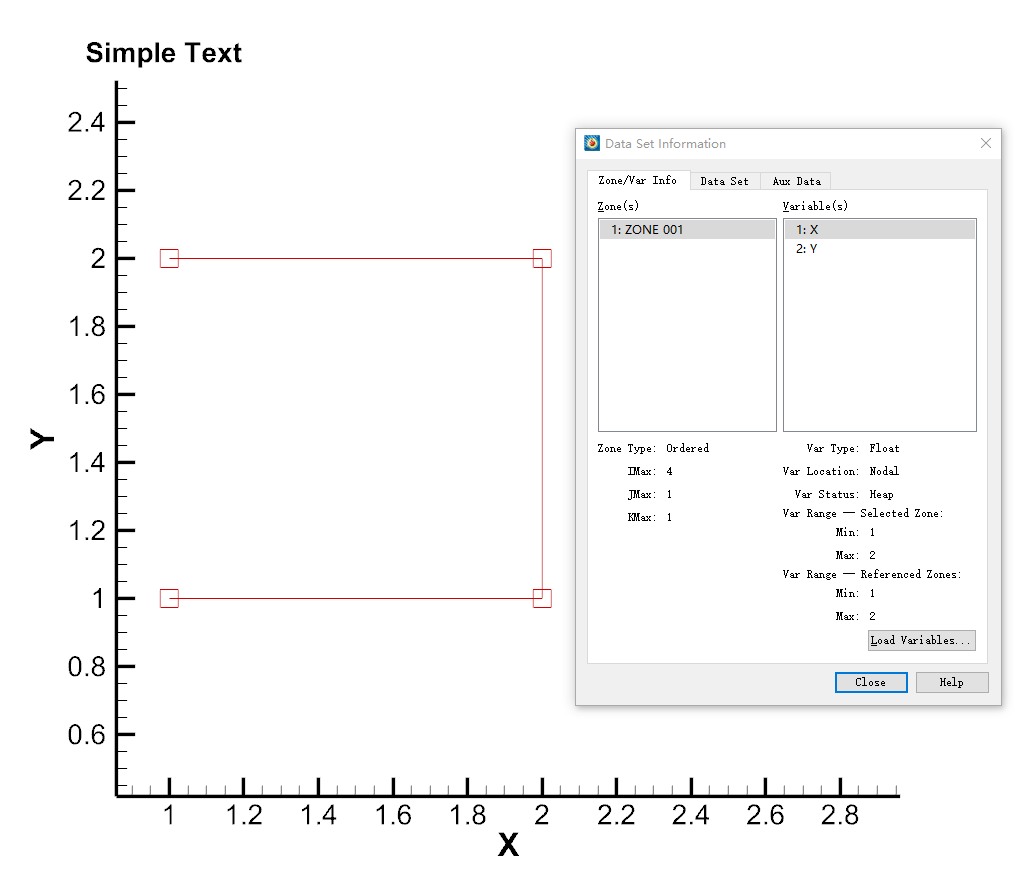
\includegraphics[width=0.7\textwidth]{example.png}
\caption{ASICC Data可视化}
\label{asiccExample}
\end{figure}

\subsection{ASCII Data的限制}
\begin{enumerate}
  \item \textbf{区数限制}:每个数据文件可以有十个自定义区,以及任意数量的文本区和几何图形区;
  \item \textbf{最大字符限制}:数据文件中一行的最大长度为32,000个字节。
\end{enumerate}

\subsection{ASCII Data的语法规则}
\begin{enumerate}
  \item \textbf{字符串}:必须使用\textcolor{red}{"}双引号\textcolor{red}{"}将带有空格或其他特殊字符的字符串括起来;
  \item \textbf{多行内容}:任何行都可以延续到一个或多个后续行(用双引号["] 括起来的文本除外);
  \item \textbf{转义符}:反斜杠(\textcolor{red}{\textbackslash})为转义符;
  \item \textbf{注释符}:井号(\textcolor{red}{\#})为注释符。
\end{enumerate}

\subsection{File Header}\label{fileHeader}
\begin{table}[!htb]
  \centering
  \caption{File Header内容}
  \begin{tabular}{*{3}{l}}
   \hline
   \textbf{项目名} & \textbf{数据格式} & \textbf{内容描述} \\
   \hline
   \texttt{TITLE} & \texttt{= <string>} & \texttt{文件名(可选)} \\
   \texttt{FILETYPE} & \texttt{= FULL, GRID or SOLUTION} & \texttt{文件类型(可选)} \\
   \texttt{VARIABLES} & \texttt{= “VARNAME1”,..., “VARNAMEN”} & \texttt{变量名} \\
   \hline
  \end{tabular}
\end{table}

\begin{lstlisting}
  TITLE = "Example File" % 项目标题
  FILETYPE = GRID % 文件类型:FULL为全类型,即包括网格与结果,FILETYPE缺省为FULL。
  VARIABLES = "X" "Y
  % 变量名:每个变量名用""包括,变量名之间用逗号、空格或换行隔开。注意顺序。
\end{lstlisting}

\subsection{Zone Record}\label{zoneRecord}
\begin{enumerate}
  \item \textbf{ZONE}:数据区关键字;
  \item \textbf{Zone Header}:数据区头文字段,描述该数据区的结构、变量名等信息,内容无顺序要求;
  \item \textbf{Data}:数据内容,与DATA PACKING和VARLOCATION的值有关;
  \item \textbf{Zone Footer}:数据区尾注,其内容与ZONETYPE有关。
\end{enumerate}

\subsubsection{Zone Header}\label{zoneHeader}
\begin{table}[!htb]
  \centering
  \caption{Zone Header内容(部分常用)}
  \begin{tabular}{*{4}{l}}
   \hline
   \textbf{项目名} & \textbf{数据格式} & \textbf{默认值} & \textbf{内容描述} \\
   \hline
   \texttt{ZONE} & \texttt{} & \texttt{} & \texttt{数据区关键字} \\
   \texttt{T} & \texttt{= <string>} & \texttt{} & \texttt{区名(可选,最长128字节)} \\
   \texttt{ZONETYPE} & \texttt{= <zonetype>} & \texttt{ORDERED} & \texttt{区类型} \\
   \texttt{I} & \texttt{= <integer>} & \texttt{} & \texttt{I方向最大点数(ORDERED用)} \\
   \texttt{J} & \texttt{= <integer>} & \texttt{} & \texttt{J方向最大点数(ORDERED用)} \\
   \texttt{K} & \texttt{= <integer>} & \texttt{} & \texttt{K方向最大点数(ORDERED用)} \\
   \texttt{NODES} & \texttt{= <integer>} & \texttt{} & \texttt{区总节点数(非ORDERED用)} \\
   \texttt{ELEMENTS} & \texttt{= <integer>} & \texttt{} & \texttt{区总单元数(非ORDERED用)} \\
   \texttt{DT} & \texttt{= (<datatype>, ...)} & \texttt{SINGLE} & \texttt{变量的数据类型,} \\
   \texttt{~} & \texttt{~} & \texttt{~} & \texttt{顺序与变量的声明顺序相同} \\
   \texttt{DATAPACKING} & \texttt{= <datapacking>} & \texttt{BLOCK} & \texttt{BLOCK(POINT)格式时,} \\
   \texttt{~} & \texttt{~} & \texttt{~} & \texttt{变量的值相继与块(点)关联} \\
   \texttt{VARLOCATION} & \texttt{=([set of vars]=} & \texttt{NODAL} & \texttt{数据位置(格心/格点)} \\
   \texttt{~} & \texttt{  <varlocation>, ...)} & \texttt{~} & \texttt{~} \\
   \texttt{STRANDID} & \texttt{= <integer>} & \texttt{} & \texttt{} \\
   \texttt{SOLUTIONTIME} & \texttt{= <double>} & \texttt{} & \texttt{求解时间} \\
   \texttt{PASSIVEVARLIST} & \texttt{= [set of vars]} & \texttt{non-passive} & \texttt{传递变量} \\
   \hline
  \end{tabular}
\end{table}

下面是两种DATAPACKING类型是文件示例,分别列出了两种情况下Zone Header应包含的内容及其格式:

示例一:DATAPACKING == POINT
\begin{lstlisting}
  ZONE T= "DATA" % 关键字与区名
  I= 37 ,J= 19 ,K= 1 % 三方向的点数、区类型默认ORDERED
  DATAPACKING=POINT
  VARLOCATION=([4,5,6]=NODAL)
\end{lstlisting}

示例二:DATAPACKING == BLOCK
\begin{lstlisting}
  ZONE T="naca0012" % 关键字与区名
  STRANDID=0, SOLUTIONTIME=0
  Nodes=32320, Elements=32000, ZONETYPE=FEQuadrilateral % 节点数、单元数、区类型
  DATAPACKING=BLOCK
  VARLOCATION=([3]=CELLCENTERED)
  DT=(DOUBLE DOUBLE DOUBLE )
\end{lstlisting}

\subsubsection{Data}\label{data}
Data存放变量的具体数值,直接跟在Zone Header后,换行隔开。数据的排布与DATAPACKING和VARLOCATION的组合相关。
\begin{lstlisting}
  DATAPACKING = BLOCK or POINT
  VARLOCATION = NODAL or CELLCENTERED
\end{lstlisting}
在BLOCK数据中,数据按变量排列(即先列出一个变量的内容,再列出之后的变量);在POINT数据中,数据按点排列(即把属于这个点的所有变量的值列出,再列出之后的点。节点或数据点,这取决于区域类型)。
在NODAL数据中,变量的值定义在每个节点(FE数据)或点(ORDERED数据)。 在CELLCENTERED数据中,变量的值定义在每个单元格(ORDERED数据)或单元(FE数据)的中心。

目前有效的组合方式为:
\begin{enumerate}
  \item BLOCK-NODAL;
  \item BLOCK-CELLCENTERED;
  \item POINT-NODAL.
\end{enumerate}

\begin{table}[!htb]
  \centering
  \caption{BLOCK数据的格式}
  \label{block}
  \begin{tabular}{*{4}{c}}
   \hline
   \texttt{A11} & \texttt{A12} & \texttt{...}  & \texttt{A1p} \\
   \texttt{A21} & \texttt{A22} & \texttt{...} & \texttt{A2p} \\
   \texttt{...} & \texttt{~} & \texttt{~} & \texttt{~} \\
   \texttt{Av1} & \texttt{Av2} & \texttt{...} & \texttt{Avp} \\
   \hline
  \end{tabular}
\end{table}
\begin{enumerate}
  \item \textbf{BLOCK-NODAL}:\\
  V为非传递、非共享的变量总数;P = I*J*K (ordered zones) or P = NODES(FE zones)
  \item \textbf{BLOCK-CELLCENTERED}:\\
  V为非传递、非共享的变量总数;P = (I - 1) * (J - 1) * (K - 1)(ordered zones) or P = ELEMENTS(FE zones)
\end{enumerate}

\begin{table}[!htb]
  \centering
  \caption{NODAL数据的格式}
  \label{nodal}
  \begin{tabular}{*{4}{c}}
   \hline
   \texttt{A11} & \texttt{A12} & \texttt{...}  & \texttt{A1v} \\
   \texttt{A21} & \texttt{A22} & \texttt{...} & \texttt{A2v} \\
   \texttt{...} & \texttt{~} & \texttt{~} & \texttt{~} \\
   \texttt{Ap1} & \texttt{Ap2} & \texttt{...} & \texttt{Apv} \\
   \hline
  \end{tabular}
\end{table}

\begin{enumerate}
  \item \textbf{POINT-NODAL}:\\
  V为非传递、非共享的变量总数;P = I * J * K(ordered zones) or P = ELEMENTS(FE zones)
\end{enumerate}

Data的通用格式要求:
\begin{enumerate}
  \item data内的数值必须用由一个或多个空格、逗号、制表符、换行符或回车分隔;
  \item 空行会被忽略;
  \item 输入值支持整形(101325)、浮点型(101325.0)及指数型(1.01325E+05);
  \item 要重复数据中的特定数字的方法为“Rep*Num”,其中Rep是重复次数,Num是要重复的某个数值。
        例如表示37个120.5的值如下所示:37*120.5。
\end{enumerate}

\subsubsection{Zone Footer}\label{zoneFooter}
Zone Footer的内容一般直接接在Data后,没有单独的关键字区分。其内容由Zone Header中的ZONETYPE确定,主要包含关联关系等内容。
\begin{enumerate}
  \item \textbf{Ordered zones}:Face Neighbor Connections List;
  \item \textbf{Cell-based finite element zones}:Connectivity information, followed by Face Neighbor Connections List;
  \item \textbf{Face-based finite element zones}:Facemap Data, followed by Boundary Map Data.
\end{enumerate}
\textcolor{red}{上述的内容在目前的算例中较少出现,这里讨论使用更多的情况Connectivity List。}

对于基于单元的有限元数据,Connectivity List一般是存放各个单元的节点标号(这个编号是Tecplot自己定义的,用来确定单元包含哪些点,
与读入的文件中所确定的点面逻辑关系不同),具体的要求为:
\begin{enumerate}
  \item 每行的关联关系对应一个单元,例如第一行对应第一个单元,以此类推;
  \item 节点编号必须按顺序给出(顺时针或逆时针);
  \item 提供的节点数应满足单元的节点数要求。
\end{enumerate}

\subsubsection{Zone Example}\label{zoneExample}
最后给出一个ASCII文件的完整结构的例子,文件用ICEM划分网格,使用Fluent计算得到结果(选取结果的一个zone)。
\begin{lstlisting}
  TITLE     = "fluent19.2.0  build-id: 10236" ------ % 项目标题
  VARIABLES = "X" ---------------------------------- % 变量名
  "Y"
  "Z"
  "Pressure"
  "X Velocity"
  "Y Velocity"
  "Z Velocity"
  DATASETAUXDATA Common.DensityVar="13" ------------ % 定义DATASETAUXDATA Common的索引
  DATASETAUXDATA Common.PressureVar="4"
  DATASETAUXDATA Common.TurbulentDynamicViscosityVar="11"
  DATASETAUXDATA Common.UVar="5"
  DATASETAUXDATA Common.VectorVarsAreVelocity="TRUE"
  DATASETAUXDATA Common.ViscosityVar="14"
  DATASETAUXDATA Common.VVar="6"
  DATASETAUXDATA Common.WVar="7"
  ZONE T="fluid" ------------------------------------ % 数据区(区名fluid)
   STRANDID=1, SOLUTIONTIME=0
   Nodes=27, Elements=8, ZONETYPE=FEBrick ----------- % fluid区的类型、节点数、单元数
   DATAPACKING=BLOCK -------------------------------- % 数据存放形式
   VARLOCATION=([4-7]=CELLCENTERED) ----------------- % 改变部分变量(4-7)的数据存放位置
   DT=(DOUBLE DOUBLE DOUBLE DOUBLE DOUBLE DOUBLE DOUBLE )
   0.000000000E+000 1.000000000E+000 0.000000000E+000 1.000000000E+000 0.000000000E+000
   1.000000000E+000 0.000000000E+000 1.000000000E+000 0.000000000E+000 1.000000000E+000
   0.000000000E+000 1.000000000E+000 0.000000000E+000 1.000000000E+000 0.000000000E+000
   1.000000000E+000 0.000000000E+000 1.000000000E+000 2.000000000E+000 2.000000000E+000
   2.000000000E+000 2.000000000E+000 2.000000000E+000 2.000000000E+000 2.000000000E+000
   2.000000000E+000 2.000000000E+000 ---------------- % "X" POINT数据
   0.000000000E+000 0.000000000E+000 1.000000000E+000 1.000000000E+000 0.000000000E+000
   0.000000000E+000 1.000000000E+000 1.000000000E+000 0.000000000E+000 0.000000000E+000
   1.000000000E+000 1.000000000E+000 2.000000000E+000 2.000000000E+000 2.000000000E+000
   2.000000000E+000 2.000000000E+000 2.000000000E+000 0.000000000E+000 1.000000000E+000
   0.000000000E+000 1.000000000E+000 0.000000000E+000 1.000000000E+000 2.000000000E+000
   2.000000000E+000 2.000000000E+000 ---------------- % "Y" POINT数据
   0.000000000E+000 0.000000000E+000 0.000000000E+000 0.000000000E+000 1.000000000E+000
   1.000000000E+000 1.000000000E+000 1.000000000E+000 2.000000000E+000 2.000000000E+000
   2.000000000E+000 2.000000000E+000 0.000000000E+000 0.000000000E+000 1.000000000E+000
   1.000000000E+000 2.000000000E+000 2.000000000E+000 0.000000000E+000 0.000000000E+000
   1.000000000E+000 1.000000000E+000 2.000000000E+000 2.000000000E+000 0.000000000E+000
   1.000000000E+000 2.000000000E+000 ---------------- % "Z" POINT数据
   1.895908591E-001 1.895908591E-001 1.895831705E-001 1.895831705E-001 7.288593259E-002
   7.288593259E-002 7.288525161E-002 7.288525161E-002 % "Pressure" CELLCENTERED数据
   4.990374637E+000 4.990374637E+000 4.990377178E+000 4.990377178E+000 5.002330072E+000
   5.002330072E+000 5.002331128E+000 5.002331128E+000 % "X Velocity" CELLCENTERED数据
   1.441273776E-007 1.441273777E-007 1.171356795E-007 1.171356796E-007 8.297792827E-007
   8.297792827E-007 7.321616937E-007 7.321616937E-007 % "Y Velocity" CELLCENTERED数据
   1.580135263E-008 -1.580135285E-008 1.580427969E-008 -1.580427966E-008 4.895852944E-008
   -4.895852947E-008 4.896084007E-008 -4.896084008E-008 % "Z Velocity" CELLCENTERED数据
   3 4 8 7 1 2 6 5 ---------------------------------- % Connectivity List
   6 8 7 5 10 12 11 9
   7 8 4 3 15 16 14 13
   11 12 8 7 17 18 16 15
   4 8 6 2 20 22 21 19
   8 12 10 6 22 24 23 21
   14 16 8 4 25 26 22 20
   16 18 12 8 26 27 24 22
\end{lstlisting}

\subsection{ASCII to Binary}\label{ascii2binary}
可以将ASCII文档转为Binary文档,可以提高读取速度。可使用Tecplot自带的preplot.exe通过命令行指令进行转换。
\textcolor{red}{注:该程序的路径为$\setminus$Tecplot$\setminus$Tecplot 360 EX 2019 R1$\setminus$bin}

对于Windows平台,下面是cmd中的等价指令,将dset.dat转为dset.plt。
\begin{lstlisting}
  preplot dset.dat dset.plt
  preplot dset
  preplot dset.dat
\end{lstlisting}


\section{Binary Data}

Binary Data的格式与ASCII Data的格式很相近,可以相互参考。不同的是,二进制文档的关键字使用逻辑判断字符,而非字符串。
此外二进制文件内没有所谓的换行。

\subsection{Binary Data的结构单元}\label{binarydataunit}
Binary Data包含两个主要的部分:header section and data section具体格式如下。
\begin{lstlisting}
  HEADER SECTION
  FLOAT32 ------------ % EOHMARKER, value=357.0
  DATA SECTION
\end{lstlisting}

\subsubsection{HEADER SECTION}\label{headersection}
二进制文件的头文件区包括:文件版本信息、项目名、变量名以及读入的所有对数据区的文本和几何定义。

\begin{lstlisting}
  i. Magic number, Version number
  #!TDVnnn ---- % 共占用8个字节, nnn为版本号,例如 #!TDV191、#!TDV112.

  ii. Integer value of 1
  INT32 ------- % 用于确定字节的读取顺序, 一般默认为1;

  iii. Title and variable names
  INT32 ------- % 文件类型 0 = FULL, 1 = GRID, 2 = SOLUTION;
  INT32*N ----- % 项目标题 N = (length of title) + 1;
  INT32 ------- % 变量数量 NumVars;
  INT32*N ----- % 变量名 N = L[1] + L[2] +...L[NumVars](L[i]为第i个变量名的长度+1).

  iv. Zones
  FLOAT32 ----- % Zone marker. Value = 299.0(v112) or 298.0(v191);
  INT32*N ----- % 数据区名 N = (length of zone name) + 1;
  INT32 ------- % ParentZone: No longer used;
  INT32 ------- % StrandID: -2 = pending strand ID for assignment by Tecplot,
                          % -1 = static strand ID,
                          % >=0 valid strand ID;
  FLOAT64 ----- % Solution time;
  INT32 ------- % 默认数据区颜色,几乎不用,默认设为-1;
  INT32 ------- % ZoneType  0=ORDERED,       1=FELINESEG,
                          % 2=FETRIANGLE,    3=FEQUADRILATERAL,
                          % 4=FETETRAHEDRON, 5=FEBRICK,
                          % 6=FEPOLYGON,     7=FEPOLYHEDRON;
  INT32 ------- % Specify Var Location (这个就是判断是不是有变量不在节点上),
                          % 0 = Don’t specify, all data is located at the nodes,
                          % 1 = Specify;

  % if “specify var location” == 1
    INT32*NV -- % 0 = Node, 1 = Cell Centered(这个顺序与之前定义变量的顺序相同,确定每个变量的储存位置);

  INT32 ------- % Are raw local 1-to-1 face neighbors supplied?(0=FALSE 1=TRUE);
  INT32 ------- % Number of miscellaneous user-defined face neighbor connections (value >= 0);
  
  % if “number of miscellaneous user-defined face neighbor connections” != 0
    INT32 ----- % User defined face neighbor mode,
                          % 0=Local 1-to-1,  1=Local 1-to-many,
                          % 2=Global 1-to-1, 3=Global 1-to-many;

    % if FE Zone
      INT32 --- % Indicates if the finite element face neighbors are completely specified by the miscellaneous,
                % face neighbors given: (0=NO, 1=YES);

  % if Ordered Zone
    INT32*3 --- % IMax, JMax, KMax(ordered类型数据的三个维度);

  % if FE Zone
    INT32 ----- % NumPts(FE类型数据的节点数);

    % if ZoneType is FEPOLYGON or FEPOLYHEDRON
      INT32/64  % NumFaces (INT32 for v112, INT64 for v191);
      INT32/64  % Total number of face nodes (INT32 for v112, INT64 for v191),
                          % (For FEPOLYGON zones, this is NumFaces*2);
      INT32 --- % Total number of boundary faces,
                          % If any boundary faces exist, include one to represent no neighboring element;
      INT32 --- % Total number of boundary connections;

    INT32 ----- % NumElements 单元数;
    INT32*3 --- % ICellDim, JCellDim, KCellDim (for future use; set to zero);

  % For all zone types (repeat for each Auxiliary data name/value pair)
    INT32 ----- % 1=Auxiliary name/value pair to follow,
                % 0=No more Auxiliary name/value pairs(结束上述的for循环);

  % If the above is 1, then supply the following
    INT32*N --- % name string (See note 1.);
    INT32 ----- % Auxiliary Value Format(Only allow 0=AuxDataType_String now);
    INT32*N --- % Value string (See note 1.).

  v. Geometries(略)

  vi. Text(略)

  vii. CustomLabel
  FLOAT32 ----- % CustomLabel Marker, F=599;
  INT32 ------- % Number of labels;
  INT32*N ----- % Text for label 1. (N=length of label + 1) See note 1;
  INT32*N ----- % Text for label 2. (N=length of label + 1) See note 1;
  .
  .
  .
  INT32*N ----- % Text for label NumLabels. (N=length of label + 1) See note 1.

  viii. UserRec
  FLOAT32 ----- % UserRec Marker; F=699;
  INT32*N ----- % Text for UserRec. See note 1.

  ix. Dataset Auxiliary data.
  FLOAT32 ----- % DataSetAux Marker; F=799.0;
  INT32*N ----- % Text for Auxiliary “Name”. See note 1;
  INT32 ------- % Auxiliary Value Format(Only allow 0=AuxDataType_String now);
  INT32*N ----- % Text for Auxiliary “Value”. See note 1.

  x. Variable Auxiliary data.
  FLOAT32 ----- % VarAux Marker; F=899.0;
  INT32*N ----- % Variable number (zero based value);
  INT32*N ----- % Text for Auxiliary “Name”. See note 1;
  INT32 ------- % Auxiliary Value Format(Only allow 0=AuxDataType_String now);
  INT32*N ----- % Text for Auxiliary “Value”. See note 1.
\end{lstlisting}

\subsubsection{DATA SECTION}\label{datasection}
DATA SECTION用于记录计算的结果。

\begin{lstlisting}
  i. For both ordered and fe zones:
  FLOAT32 ----- % Zone marker Value = 299.0 for v112,
                % Zone marker Value = 298.0 for v191;
  INT32*N ----- % Variable data format, N=Total number of vars,
                        % 1=Float,    2=Double, 3=LongInt,
                        % 4=ShortInt, 5=Byte,   6=Bit;
  INT32 ------- % Has passive variables: 0 = no, 1 = yes;

  % if “has passive variables” != 0
    INT32*NV -- % Is variable passive: 0 = no, 1 = yes,
                % (Omit entirely if “Has passive variables” is 0);

  INT32 ------- % Has variable sharing 0 = no, 1 = yes;

  % if “has variable sharing” != 0
    INT32*NV -- % Zero based zone number to share variable with (relative to this datafile),
                % (-1=no sharing),(Omit entirely if “Has variable sharing”=0);

  INT32 ------- % Zero based zone number to share connectivity list with (-1 = no sharing);
  
  % Compressed list of min/max pairs for each non-shared and non-passive variable. 
  % For each non-shared and non-passive variable (as specified above)
    FLOAT64 --- % Min value; (按变量定义的顺序遍历其最大值与最小值)
    FLOAT64 --- % Max value;

  xxxxxxxxxx -- % Zone Data. Each variable is in data format as specified above.
                % 最后这里是具体数据,数据类型按照之前的规定,换变量直接跟随。对应Tecplot Spreadsheet中的内容。

  ii. specific to ordered zones
  % if “zone number to share connectivity list with” == -1 &&
  %    “num of misc. user defined face neighbor connections” != 0
    INT32*N --- % Face neighbor connections,
                % N = (number of miscellaneous user defined face neighbor connections) * P,
                % (See note 5);

  iii. specific to fe zones when FileType is not SOLUTION
  % if ZoneType is NOT FEPOLYGON or FEPOLYHEDRON

    % if “zone number to share connectivity lists with” == -1
      INT32*N - % Zone Connectivity Data N=L*JMax (see note 2);
                % (这里是zero base 和ASCII文件相应部分对比数值上少1)

    % if “zone number to share connectivity lists with” == -1 &&
    %    “raw local 1-to-1 face neighbors are supplied”
      INT32*N - % Raw local 1-to-1 face neighbor array,
                % N = (NumElements * NumFacesPerElement), (See note 3);

    % if “zone number to share connectivity lists with” == -1 &&
    %    “num of misc. user defined face neighbor connections” != 0
      INT32*N - % Face neighbor connections,
                % N = (number of miscellaneous user defined face neighbor connections) * P,
                % (See note 4);

  % if ZoneType is FEPOLYGON or FEPOLYHEDRON
    % if “zone number to share face map data with” == -1
      % if the zone header version for this zone is v112
        INT32*(F+1) --- % Face node offsets into the face nodes array below,
                        % Does not exist for FEPOLYGON zones. F = NumFaces;

      % elseif the zone header version for this zone is v191
        INT32*F --- % Face node count for each face,
                    % Does not exist for FEPOLYGON zones. F = NumFaces;

      INT32*FN ---- % Face nodes array containing the node numbers for all nodes in all faces,
                    % FN = total number of face nodes;
      INT32*F ----- % Elements on the left side of all faces. F = NumFaces;
      INT32*F ----- % Elements on the right side of all faces. F = NumFaces;

      % if “total number of boundary faces” != 0
        INT32*NBF - % Boundary face connection offsets into the boundary face connecion elements array 
                    % and the boundary face connection zones array. NBF = total number of boundary faces + 1;
        INT32*NBI - % Boundary face connection elements. NBI = total number of boundary connections;
        INT32*NBI - % Boundary face connection zones. NBI = total number of boundary connections.
\end{lstlisting}

\subsubsection{NOTES}\label{notes}
这里是Tecplot数据格式手册的注释,保留原文参考。
\begin{enumerate}
  \item 
  All character data is represented by INT32 values.Example: The letter “A” has an ASCII value of 65. 
  The WORD written to the data file for the letter “A” is then 65.
  
  All character strings are null terminated
 (i.e. terminated by a zero value)

 \item 
 This represents JMax sets of adjacency zero based indices where each\\
 set contains L values and L is\\
 2 for LINESEGS\\
 3 for TRIANGLES\\
 4 for QUADRILATERALS\\
 4 for TETRAHEDRONS\\
 8 for BRICKS

 \item 
 The raw face neighbor array is dimensioned by (number of elements for the zone) times 
 (the number of faces per element), where each member of the array holds the zero-based element neighbor of that face. 
 A boundary face is one that has no neighboring element and is represented by a -1. 
 Faces should only be neighbors if they logically share nodes and they should be reciprocal.
 \item note 4
 \begin{table}[!htb]
  \centering
  \begin{tabular}{*{3}{l}}
   \texttt{FaceNeighbor Mode} & \texttt{values} & \texttt{Data} \\
   \hline
   \texttt{LocalOneToOne} & \texttt{3} & \texttt{cz,fz,cz} \\
   \texttt{LocalOneToMany} & \texttt{nz+4} & \texttt{cz,fz,oz,nz,cz1,cz2,...,czn} \\
   \texttt{GlobalOneToOne} & \texttt{4} & \texttt{cz,fz,ZZ,CZ} \\
   \texttt{GlobalOneToMany} & \texttt{2*nz+4} & \texttt{cz,fz,oz,nz,ZZ1,CZ1,ZZ2,CZ2,...,ZZn,CZn} \\
   \hline
  \end{tabular}
\end{table}

\begin{table}[!htb]
  \centering
  \begin{tabular}{*{1}{l}}
   \texttt{Where:} \\
   \texttt{  cz = cell in current zone (zero based)} \\
   \texttt{  fz = face of cell in current zone (zero based)} \\
   \texttt{  oz = face obscuration flag (only applies to one-to-many):} \\
   \texttt{    0 = face partially obscured} \\
   \texttt{    1 = face entirely obscured} \\
   \texttt{  nz = number of cell or zone/cell associations} \\
   \texttt{    (only applies to one-to-many)} \\
   \texttt{  ZZ = remote Zone (zero based)} \\
   \texttt{  CZ = cell in remote zone (zero based)} \\
   \end{tabular}
\end{table}
 cz,fz combinations must be unique and multiple entries are not allowed. 
 Additionally, Tecplot assumes that with the one-to-one face neighbor modes, 
 a supplied cell face is entirely obscured by its neighbor. 
 With one-to-many, the obscuration flag must be supplied.
 Face neighbors that are not supplied are run through
 Tecplot’s auto face neighbor generator (FE only).

 \item 
 Cell centered variable (DATA SECTION)\\
 To make reading of cell centered binary data efficient, Tecplot stores
 IMax*JMax*(KMax-1) numbers of cell centered values, where IMax, JMax,
 and KMax represent the number of points in the I, J, and K directions.
 Therefore extra zero values (ghost values) are written to the data file
 for the fastest moving indices. For example, if your data's IJK
 dimensions are 2x3x2, a cell-centered variable will have 1x2x1
 (i.e. (I-1)x(J-1)x(K-1)) significant values. However, 2x3x1 values must
 be written out because it must include the ghost values. Assume that the
 two significant cell-centered values are 1.5 and 12.5. The ghost values
 will be output with a zero value.\\
 So if the zone was dimensioned 2x3x2 its cell centered variable would be
 represented as follows:\\
 1.5 0.0 12.5 0.0 0.0 0.0\\
 If the zone was dimensioned 3x2x2 its cell centered variable would be
 represented as follows:\\
 1.5 12.5 0.0 0.0 0.0 0.0\\
 and if the zone was dimensioned 2x2x3 its cell centered variable would be
 represented as follows:\\
 1.5 0.0 0.0 0.0 12.5 0.0 0.0 0.0\\
 For large variables the wasted space is less significant that it
 is for the small example above.
\end{enumerate}

\section{附录}

\subsection{Index检索}
\begin{enumerate}[label=\arabic*).]
  \item ASCII Data 关键字; \upref{keyword}
  \item ASCII Data 常用Zone Header; \upref{zoneHeader}
  \item ASCII Data BLOCK数据的格式; \upref{block}
  \item ASCII Data NODAL数据的格式; \upref{nodal}
  \item Binary Data 结构单元; \upref{binarydataunit}
  \item Binary Data HEADER SECTION; \upref{headersection}
  \item Binary Data DATA SECTION. \upref{datasection}
\end{enumerate}

\end{document}